\documentclass[12pt, a4paper]{article}

% ===============================
% Packages (no duplicates)
% ===============================
\usepackage{fontspec}
\usepackage{xeCJK}
\usepackage{amsmath, amssymb}
\usepackage{graphicx}
\usepackage{geometry}
\usepackage{tikz}

\geometry{margin=1in}

% ===============================
% Font Setup
% ===============================
\setmainfont{TeX Gyre Termes}
\setsansfont{TeX Gyre Heros}
\setmonofont{Latin Modern Mono}
\setCJKmainfont{Noto Serif CJK TC}

% ===============================
% TikZ Libraries
% ===============================
\usetikzlibrary{3d, arrows.meta}

\title{Magnetic Flux Through a Circular Loop}
\author{}
\date{}

\begin{document}

\maketitle

% ==========================================================
\section{Problem Statement}

A circular loop of radius $b$ lies in the $xy$-plane.  
The magnetic field is given by

\[
\mathbf{B} = \mathbf{a}_z B_0 
\cos\!\left(\frac{\pi r}{2b}\right)
\sin(\omega t)
\]

We compute the magnetic flux:

\[
\Phi = \int_S \mathbf{B} \cdot d\mathbf{s}
\]

% ==========================================================
\section{Surface Element in Polar Coordinates}

In polar coordinates, the scalar surface element is

\[
dA = r\,dr\,d\theta
\]

Since the surface normal is in the $z$-direction,

\[
d\mathbf{s} = \mathbf{a}_z r\,dr\,d\theta
\]

Because $\mathbf{B}$ is independent of $\theta$, integrate $\theta$ from $0$ to $2\pi$:

\[
\int_0^{2\pi} r\,dr\,d\theta
=
r\,dr \int_0^{2\pi} d\theta
=
2\pi r\,dr
\]

Thus,

\[
d\mathbf{s} = \mathbf{a}_z\,2\pi r\,dr
\]

% ==========================================================
\section{Flux Calculation}

\[
\Phi
=
\int_0^b
B_0 
\cos\!\left(\frac{\pi r}{2b}\right)
\sin(\omega t)
\,(2\pi r\,dr)
\]

\[
\Phi
=
2\pi B_0 \sin(\omega t)
\int_0^b
r \cos\!\left(\frac{\pi r}{2b}\right) dr
\]

Evaluating the integral:

\[
\Phi
=
\frac{8b^2}{\pi}
\left(
\frac{\pi}{2} - 1
\right)
B_0 \sin(\omega t)
\]

% ==========================================================
\section{Geometric Interpretation Using TikZ}

\begin{center}
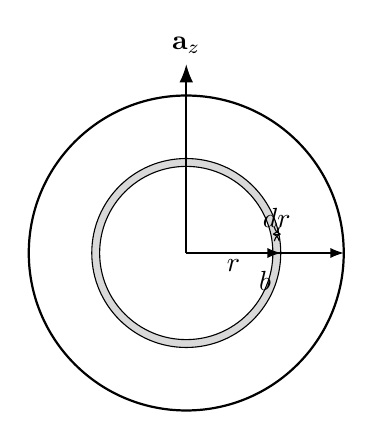
\begin{tikzpicture}[scale=2]

% Outer circle (radius b)
\draw[thick] (0,0) circle (1);

% Differential ring (shaded)
\draw[fill=gray!30] (0,0) circle (0.6);
\draw[fill=white] (0,0) circle (0.55);

% Radius r
\draw[-{Latex}] (0,0) -- (0.6,0);
\node at (0.3,-0.08) {$r$};

% Thickness dr
\draw[<->] (0.55,0.12) -- (0.6,0.12);
\node at (0.575,0.22) {$dr$};

% Radius b
\draw[-{Latex}] (0,0) -- (1,0);
\node at (0.5,-0.18) {$b$};

% z direction
\draw[-{Latex}, thick] (0,0) -- (0,1.2);
\node at (0,1.32) {$\mathbf{a}_z$};

\end{tikzpicture}
\end{center}

The shaded region represents a thin circular ring:

\[
dA = (2\pi r)(dr)
\]

Thus,

\[
d\mathbf{s} = \mathbf{a}_z\, 2\pi r\, dr
\]

% ==========================================================
\section{Geometric Shape of the Surface}

The circular loop of radius $b$ lies in the $xy$-plane.  
The surface bounded by the loop is chosen as the flat disk:

\[
x^2 + y^2 \le b^2, \quad z = 0.
\]

This is a \textbf{flat circular disk} located in the $xy$-plane.

The unit normal vector is:

\[
\hat{n} = \mathbf{a}_z
\]

which points in the positive $z$-direction.

% ==========================================================
\section{3D Visualization Using TikZ}

\begin{center}
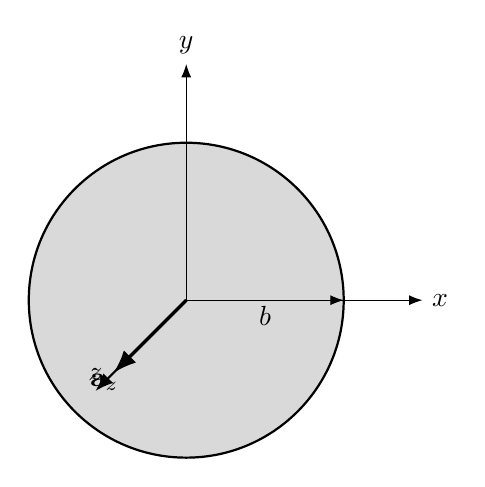
\begin{tikzpicture}[scale=2]

% 3D coordinate setup
\begin{scope}[canvas is xy plane at z=0]
    % Filled disk
    \fill[gray!30] (0,0) circle (1);
    % Boundary circle
    \draw[thick] (0,0) circle (1);
\end{scope}

% Axes
\draw[-{Latex}] (0,0,0) -- (1.5,0,0) node[right] {$x$};
\draw[-{Latex}] (0,0,0) -- (0,1.5,0) node[above] {$y$};
\draw[-{Latex}, thick] (0,0,0) -- (0,0,1.5) node[above] {$z$};

% Normal vector
\draw[-{Latex}, very thick] (0,0,0) -- (0,0,1.2);
\node at (0,0,1.35) {$\mathbf{a}_z$};

% Radius b
\draw[-{Latex}] (0,0,0) -- (1,0,0);
\node at (0.5,-0.1,0) {$b$};

\end{tikzpicture}
\end{center}

% ==========================================================
\section{Mathematical Description}

The surface can be parameterized using polar coordinates:

\[
\mathbf{r}(r,\theta) =
(r\cos\theta,\; r\sin\theta,\; 0)
\]

where

\[
0 \le r \le b, \quad 0 \le \theta \le 2\pi.
\]

The differential surface element is:

\[
dS = r\,dr\,d\theta
\]

and the vector surface element is:

\[
d\mathbf{s} = \mathbf{a}_z\, r\,dr\,d\theta.
\]

% ==========================================================
\section{Introduction to the Faraday Disk Generator}

The Faraday disk generator (also called a homopolar generator) consists of a 
conducting disk rotating in a uniform magnetic field. 
Electrical contacts are made at the center and the rim of the disk, forming 
a closed external circuit.

The system demonstrates \textbf{motional electromotive force (EMF)} produced 
by the Lorentz force acting on moving charges.

\section{Physical Setup}

\begin{itemize}
\item A conducting circular disk
\item Angular velocity $\omega$
\item Uniform magnetic field $B$ perpendicular to the disk
\item Electrical contacts at the center and rim
\end{itemize}

\subsection{Faraday Disk Geometry}

\begin{center}
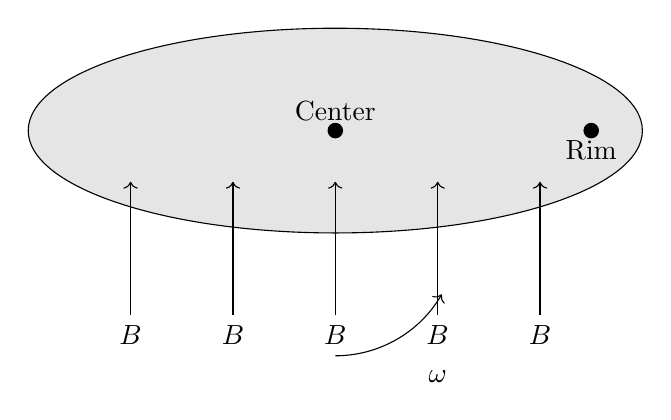
\begin{tikzpicture}[scale=1.3]

% Disk
\draw[fill=gray!20] (0,0) ellipse (3 and 1);

% Center
\filldraw (0,0) circle (2pt);
\node[above] at (0,0) {Center};

% Rim point
\filldraw (2.5,0) circle (2pt);
\node[below] at (2.5,0) {Rim};

% Magnetic field arrows
\foreach \x in {-2,-1,0,1,2}
{
\draw[->] (\x,-1.8) -- (\x,-0.5);
\node at (\x,-2) {$B$};
}

% Rotation arrow
\draw[->] (0,-2.2) arc (-90:-30:1.2);
\node at (1,-2.4) {$\omega$};

\end{tikzpicture}
\end{center}

\section{Velocity of Charges}

A point on the disk at radius $r$ moves with tangential velocity

\[
v = \omega r
\]

where

\begin{itemize}
\item $\omega$ is the angular velocity
\item $r$ is the distance from the center
\end{itemize}

\section{Lorentz Force}

Charges moving in a magnetic field experience the Lorentz force

\[
\vec{F} = q(\vec{v} \times \vec{B})
\]

Since $\vec{v}$ is tangential and $\vec{B}$ is vertical, the force points
radially outward.

Therefore electrons are pushed from the center toward the rim.

\section{Electric Field in the Disk}

The motional electric field produced inside the conductor is

\[
E = vB
\]

Substituting $v=\omega r$ gives

\[
E = \omega r B
\]

The electric field points radially outward.

\section{Generated Voltage}

The voltage between the center and rim is obtained by integrating the electric field:

\[
V_0 = \int_0^R E\,dr
\]

Substituting the electric field:

\[
V_0 = \int_0^R \omega B r \, dr
\]

\[
V_0 = \frac{1}{2} B \omega R^2
\]

\section{Current Loop in Three Dimensions}

The complete current path forms a closed loop consisting of:

\begin{enumerate}
\item center contact
\item radial path through the disk
\item rim contact
\item external wire
\item return to the center
\end{enumerate}

\subsection{3D Current Loop Concept}

\begin{center}
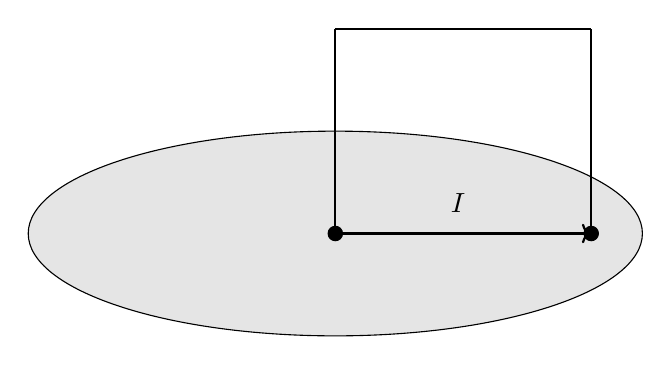
\begin{tikzpicture}[scale=1.3]

% Disk
\draw[fill=gray!20] (0,0) ellipse (3 and 1);

% Center
\filldraw (0,0) circle (2pt);

% Rim
\filldraw (2.5,0) circle (2pt);

% Radial current
\draw[->, thick] (0,0) -- (2.5,0);

% External wire
\draw[thick] (2.5,0) -- (2.5,2);
\draw[thick] (2.5,2) -- (0,2);
\draw[thick] (0,2) -- (0,0);

\node at (1.2,0.3) {$I$};

\end{tikzpicture}
\end{center}

\section{Current Distribution in the Disk}

The current does not flow along a single radial line. 
Instead, it spreads across the entire conducting surface of the disk.

Thus the disk behaves like many parallel radial conductors.

\subsection{Radial Current Flow}

\begin{center}
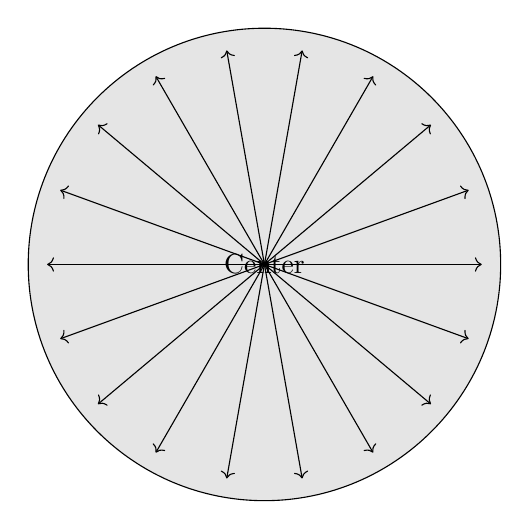
\begin{tikzpicture}[scale=1.2]

% Disk
\draw[fill=gray!20] (0,0) circle (2.5);

% Radial arrows
\foreach \angle in {0,20,...,340}
{
\draw[->] (0,0) -- (\angle:2.3);
}

\node at (0,0) {Center};

\end{tikzpicture}
\end{center}

The current density spreads radially outward from the center to the rim.

\section{Magnetic Flux Consideration}

In this system the magnetic field is constant:

\[
\frac{d\Phi}{dt} = 0
\]

Yet an EMF appears. This occurs because the EMF arises from the motion
of the conductor in the magnetic field.

The general EMF expression is

\[
\mathcal{E} = \oint (\vec{E} + \vec{v} \times \vec{B}) \cdot d\vec{l}
\]

In the Faraday disk generator, the EMF is produced by the term

\[
\vec{v} \times \vec{B}
\]

\section{Conclusion}

The Faraday disk generator demonstrates that voltage can be produced
by moving conductors in a magnetic field.

Key results:

\begin{itemize}
\item Charges experience the Lorentz force
\item Current flows radially through the disk
\item The generated voltage is
\[
V_0 = \frac{1}{2} B \omega R^2
\]
\end{itemize}
\section{Magnetic Flux Definition}

The magnetic flux through a surface $S$ is defined as

\begin{equation}
\Phi = \int_S \mathbf{B}\cdot d\mathbf{s}
\end{equation}

where

\begin{itemize}
\item $\mathbf{B}$ is the magnetic field
\item $d\mathbf{s}$ is the differential surface vector
\end{itemize}

We want to compute the time derivative of the flux.

\begin{equation}
\frac{d\Phi}{dt} = \frac{d}{dt}\int_S \mathbf{B}\cdot d\mathbf{s}
\end{equation}

In general, both the magnetic field and the surface may change with time.

\section{Flux Difference Over a Small Time Interval}

Consider a small time increment $\Delta t$.

\begin{itemize}
\item $S_1$ is the surface at time $t$
\item $S_2$ is the surface at time $t+\Delta t$
\end{itemize}

Then

\begin{equation}
\frac{d\Phi}{dt}
=
\lim_{\Delta t\rightarrow0}
\frac{1}{\Delta t}
\left[
\int_{S_2}\mathbf{B}(t+\Delta t)\cdot d\mathbf{s}_2
-
\int_{S_1}\mathbf{B}(t)\cdot d\mathbf{s}_1
\right]
\end{equation}

\section{Taylor Expansion of the Magnetic Field}

The magnetic field at time $t+\Delta t$ can be expanded using a Taylor series:

\begin{equation}
\mathbf{B}(t+\Delta t)
=
\mathbf{B}(t)
+
\frac{\partial \mathbf{B}}{\partial t}\Delta t
+
\text{H.O.T.}
\end{equation}

where H.O.T. represents higher order terms in $\Delta t$.

\section{Substituting into the Flux Expression}

Substitute the Taylor expansion into the flux integral:

\begin{equation}
\int_{S_2}
\left[
\mathbf{B}(t)
+
\frac{\partial \mathbf{B}}{\partial t}\Delta t
\right]
\cdot d\mathbf{s}_2
\end{equation}

Split the integral:

\begin{equation}
=
\int_{S_2}\mathbf{B}(t)\cdot d\mathbf{s}_2
+
\Delta t
\int_{S_2}
\frac{\partial \mathbf{B}}{\partial t}\cdot d\mathbf{s}_2
\end{equation}

\section{Divide by $\Delta t$}

Substituting back into the flux derivative gives

\begin{align}
\frac{d}{dt}\int_S \mathbf{B}\cdot d\mathbf{s}
&=
\int_S \frac{\partial \mathbf{B}}{\partial t}\cdot d\mathbf{s}
\\
&+
\lim_{\Delta t\rightarrow0}
\frac{1}{\Delta t}
\left[
\int_{S_2}\mathbf{B}\cdot d\mathbf{s}_2
-
\int_{S_1}\mathbf{B}\cdot d\mathbf{s}_1
\right]
\end{align}

\section{Physical Meaning of the Two Terms}

The result separates into two contributions.

\subsection{Time-Varying Magnetic Field}

\begin{equation}
\int_S \frac{\partial \mathbf{B}}{\partial t}\cdot d\mathbf{s}
\end{equation}

This term represents the flux change caused by a magnetic field that varies with time.

\subsection{Motion of the Surface}

\begin{equation}
\lim_{\Delta t\rightarrow0}
\frac{1}{\Delta t}
\left[
\int_{S_2}\mathbf{B}\cdot d\mathbf{s}_2
-
\int_{S_1}\mathbf{B}\cdot d\mathbf{s}_1
\right]
\end{equation}

This term arises because the surface itself moves in the magnetic field.

\section{Connection to Faraday's Law}

For a moving circuit, the final result leads to the general form of Faraday's law

\begin{equation}
\oint_C \mathbf{E}\cdot d\mathbf{l}
=
-
\int_S \frac{\partial \mathbf{B}}{\partial t}\cdot d\mathbf{s}
+
\oint_C (\mathbf{u}\times\mathbf{B})\cdot d\mathbf{l}
\end{equation}

where

\begin{itemize}
\item $\mathbf{u}$ is the velocity of the conductor
\item the second term represents the motional electromotive force
\end{itemize}

\section{Summary}

The time derivative of magnetic flux separates into two effects:

\begin{enumerate}
\item Change of the magnetic field with time
\item Motion of the surface in a magnetic field
\end{enumerate}

This decomposition explains the origin of both transformer EMF and motional EMF.
\section{Introduction}

When an external electric field is applied to a material, the positive and negative charges inside atoms shift slightly. This separation of charge creates microscopic electric dipoles throughout the material.

This phenomenon is called \textbf{polarization}.

\section{Microscopic Picture}

Without an external electric field, the center of the electron cloud and the nucleus coincide.

\subsection{No Electric Field}

\begin{center}
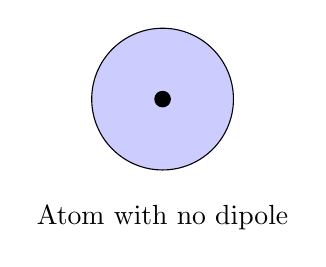
\begin{tikzpicture}[scale=1.5]

\draw[fill=blue!20] (0,0) circle (0.6);
\fill (0,0) circle (2pt);
\node at (0,-1) {Atom with no dipole};

\end{tikzpicture}
\end{center}

\subsection{With Electric Field}

When an electric field $E$ is applied, the electron cloud shifts slightly opposite to the field direction.

\begin{center}
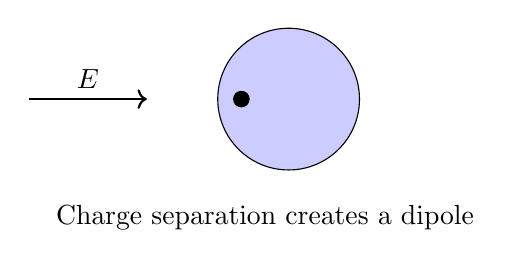
\begin{tikzpicture}[scale=1.5]

\draw[->,thick] (-2,0) -- (-1,0) node[midway,above] {$E$};

\draw[fill=blue!20] (0.2,0) circle (0.6);
\fill (-0.2,0) circle (2pt);

\node at (0,-1) {Charge separation creates a dipole};

\end{tikzpicture}
\end{center}

This separation forms a dipole moment

\[
\mathbf{p} = q\mathbf{d}
\]

where $q$ is the charge and $d$ is the separation distance.

\section{Polarization Vector}

Polarization is defined as the dipole moment per unit volume:

\[
\mathbf{P} = \frac{\text{total dipole moment}}{\text{volume}}
\]

The unit of polarization is

\[
[C/m^2]
\]

\section{Polarization in Materials}

Inside a material, many dipoles appear and align with the electric field.

\begin{center}
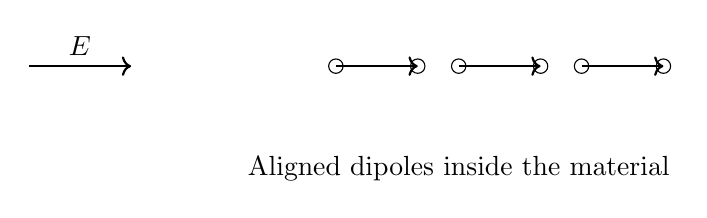
\begin{tikzpicture}[scale=1.3]

\draw[->,thick] (-3,0) -- (-2,0) node[midway,above] {$E$};

\foreach \x in {0,1.2,2.4}
{
\draw[->,thick] (\x,0) -- (\x+0.8,0);
\draw (\x,0) circle (2pt);
\draw (\x+0.8,0) circle (2pt);
}

\node at (1.2,-1) {Aligned dipoles inside the material};

\end{tikzpicture}
\end{center}

\section{Bound Charges}

Polarization produces bound charges in the material.

Surface bound charge density:

\[
\sigma_b = \mathbf{P} \cdot \hat{n}
\]

Volume bound charge density:

\[
\rho_b = - \nabla \cdot \mathbf{P}
\]

\section{Relation with Electric Displacement Field}

Maxwell introduced the electric displacement field:

\[
\mathbf{D} = \varepsilon_0 \mathbf{E} + \mathbf{P}
\]

This allows Maxwell's equations to be written in terms of \textbf{free charge} instead of total charge.

\section{Linear Dielectric Materials}

For linear materials,

\[
\mathbf{P} = \varepsilon_0 \chi_e \mathbf{E}
\]

so

\[
\mathbf{D} = \varepsilon \mathbf{E}
\]

where

\[
\varepsilon = \varepsilon_0 (1 + \chi_e)
\]

\section{Summary}

Polarization describes how electric fields slightly separate positive and negative charges inside matter, producing microscopic dipoles. The collective effect of these dipoles determines the macroscopic electromagnetic behavior of materials.

\end{document}